\section{Catalog of real-time mitigation techniques}
\label{section:hardware:catalog}

\subsection{Existing real-time implementations}
\label{subsection:hardware:catalog:existing}
\subsubsection{Preventive : Avoidance ASKAP(?) (Greg, Benjamin)}
\subsubsection{Analog: Adaptive analog attenuators LWA (Greg)}
\subsection{Analog: GMRT (Kaushal)}
\subsubsection{Digital: Excision in time MAD filter GMRT (Kaushal}
\subsubsection{Digital: Excision in spectral}
\begin{itemize}
\item AOFlagger-type Westerbork (Greg)

 RFIm \cite{sclocco2019real} is an open-source, high-performance library designed to mitigate RFI in real time. RFIm is optimized to run on many-core accelerators such as GPUs and provides methods that are robust yet computationally efficient. The library features two main algorithms : Time-Domain Sigma Cut (TDSC) and Frequency-Domain Sigma Cut (FDSC). These two algorithms detect and replace RFI-contaminated data with statistical averages to reduce false positives without significant impact on processing time. This approach allows systems like the Apertif Radio Transient System (ARTS) to maintain high data throughput while effectively identifying real astronomical signals amidst increasing anthropogenic and satellite-generated interference.
 
\item Higher-order statistics at EOVSA (Greg)

The Spectral Kurtosis (SK) technique is a statistical method used for real-time detection of non-Gaussian signals, such as radio frequency interference (RFI), within Gaussian noise in radio astronomy data. The SK estimator distinguishes signals by comparing power and power-squared values of spectral data to detect deviations from Gaussian behavior. The Expanded Owens Valley Solar Array (EOVSA) implements this SK technique in its correlator, using an FPGA-based system to perform real-time SK calculations directly within the Fourier transform engine \cite{}. This design allows the system to flag and exclude contaminated data dynamically, enhancing the quality of observations by effectively identifying and mitigating RFI while preserving genuine astronomical signals.

\item Frequency and Time Median filter on Nancay Decameter Array (Cedric)

Will describe here a receiver that operates in the 10-35 MHz band for solar and Jovian daily observations since 2015 (?).

It implements a classical (averaged-based) time-frequency analysis using a Welch averaged periodogram and simultaneously computes the same periodogram with a median filter applied on the frequency axis first and then on the time axis to mitigate narrow-band and wide-band RFI from observations.

\item RFI mitigation implementations on RDH at Nançay (Cedric)

Will describe here :
\begin{itemize}
\item a time domain impulse detector based on a power criterion to mitigate L-band radar system radio echoes with excision of time domain data.  Such RFI is used to impair observations of red-shifted HI galaxies observed at the Nançay Decimeter Radiotelescope.
\item a time-frequency domain based on a MAD-estimated power criterion to mitigate Iridium constellation space-to-earth downlinks.  Such RFI was used to impair observations of 1667-MHz red-shifted OH line from mega-maser that would fall near 1622\ MHz.
\end{itemize}


\item CHIME (Thushara)
\end{itemize}

\subsection{Prospective real-time implementations}
\label{subsection:hardware:catalog:prospective}

\subsubsection{Preventive : Dynamic scheduler (Greg)}
\subsection{Analog: Notch filters for uGMRT (Kaushal)}
\subsubsection{Analog : Tunable notch filter DSA-2000 (Greg)}

The tunable notch filters are designed to mitigate RFI in the analog front-end of the DSA-2000 receivers. The Quad-Stub Resonator Filter uses four high-Q “series LC” stubs, each controlled by voltage-tuned varactors, allowing independent frequency tuning for precise RFI mitigation. The filter achieves deep notch attenuation, adjustable within a range of 550 MHz to 1050 MHz, with peak attenuation up to 62.5 dB. It features a chassis design with RFI-tight seals and SMA connectors to prevent interference coupling. The filter's response is fine-tuned through individual varactor bias adjustments, enabling adaptable and effective RFI suppression across a broad frequency range.

\subsubsection{Analog : Reconfigurable Intelligent Surface (Greg)}

Reconfigurable Intelligent Surfaces (RIS) can mitigate RFI at the telescope receiver by dynamically shaping the electromagnetic wavefronts to create a destructive interference zone around the receiver \cite{zou2022scisrs,wei2024ris,wei2023multistage}. The RIS array, composed of multiple controllable elements, adjusts the phase and amplitude of reflected signals to precisely counteract incoming RFI. By steering reflected signals from the RIS in such a way that they are out of phase with the incident RFI, the RIS effectively cancels the RFI energy before it reaches the telescope’s receiver. This approach allows for the creation of an electromagnetic quiet zone, enabling the telescope to perform sensitive astronomical observations without interference from external RFI sources, such as aircraft and satellites, without altering the telescope’s primary astronomical signals.

\subsubsection{Digital : Excision in time parametric subtraction ellingson (Greg)}

The time-domain coherent cancellation (CTC) technique is a method used to mitigate RFI by subtracting an interference estimate from the received signal in real time \cite{ellingson2022coherent}. CTC operates by generating a reference signal that represents the interfering source, which can be acquired externally (e.g., through a separate antenna) or synthesized internally using prior knowledge of the interference. The reference signal is used to create an interference estimate that is coherently subtracted from the received signal, ideally leaving only the astronomical signal of interest with minimal added noise or distortion. The approach allows telescopes to "look through" interference, preserving affected data that would otherwise be discarded by traditional methods, though it requires precise estimation and synchronization to avoid errors that could compromise the scientific data.

\subsubsection{Digital : Threshold-based pre-correlation RFI detection technique to be used in SKA.Mid (Thushara)}
\label{subsection:hardware:catalog:ska-mid}

The Correlator Beamformer for the Mid-frequency telescope for the Square Kilometre Array (SKA-Mid.CBF) is to use 'power threshold-based' RFI detection scheme. The main objective is to preserve the linearity of the signal chain while achieving the desired dynamic range to maintain the sensitivity. The architecture of the proposed RFI detector/flagger module is shown in Figure~\ref{fig:rfi_df_ska_mid_cbf}. As shown there, two time scales are involved:
\begin{enumerate}
    \item Long-term ($>$1 sec, considering on/off state of the noise diode) for establishing an average power level, and
    \item Short-term to detect and flag bursting RFI to prevent downstream spectral splatter.
\end{enumerate}

The number of samples used for the short-term power calculation is programmable. If the short-term power calculation is greater than a programmable threshold, set by the Telescope-Manage or internally determined if “auto-set”, then a flag is set and carried with the data stream to the downstream processing module, and downstream operations (i.e. any that affect output data products or intermediate calculations needed such as gains/levels settings) are inhibited for the number of samples that it takes the flag to propagate through all downstream processing modules. As per the flagging policy, both polarization components are flagged if one is flagged. The dwell time of the flag is also programmable to balance the data loss with the risk of contamination. Note that the flagged data is not used in evaluating the long-term power calculation in order to have an estimate of the signal level of non-RFI-contaminated signal. The long-term power is accumulated in two separate bins, one for noise diode on, and one for noise diode off.

\begin{figure}
    \centering
    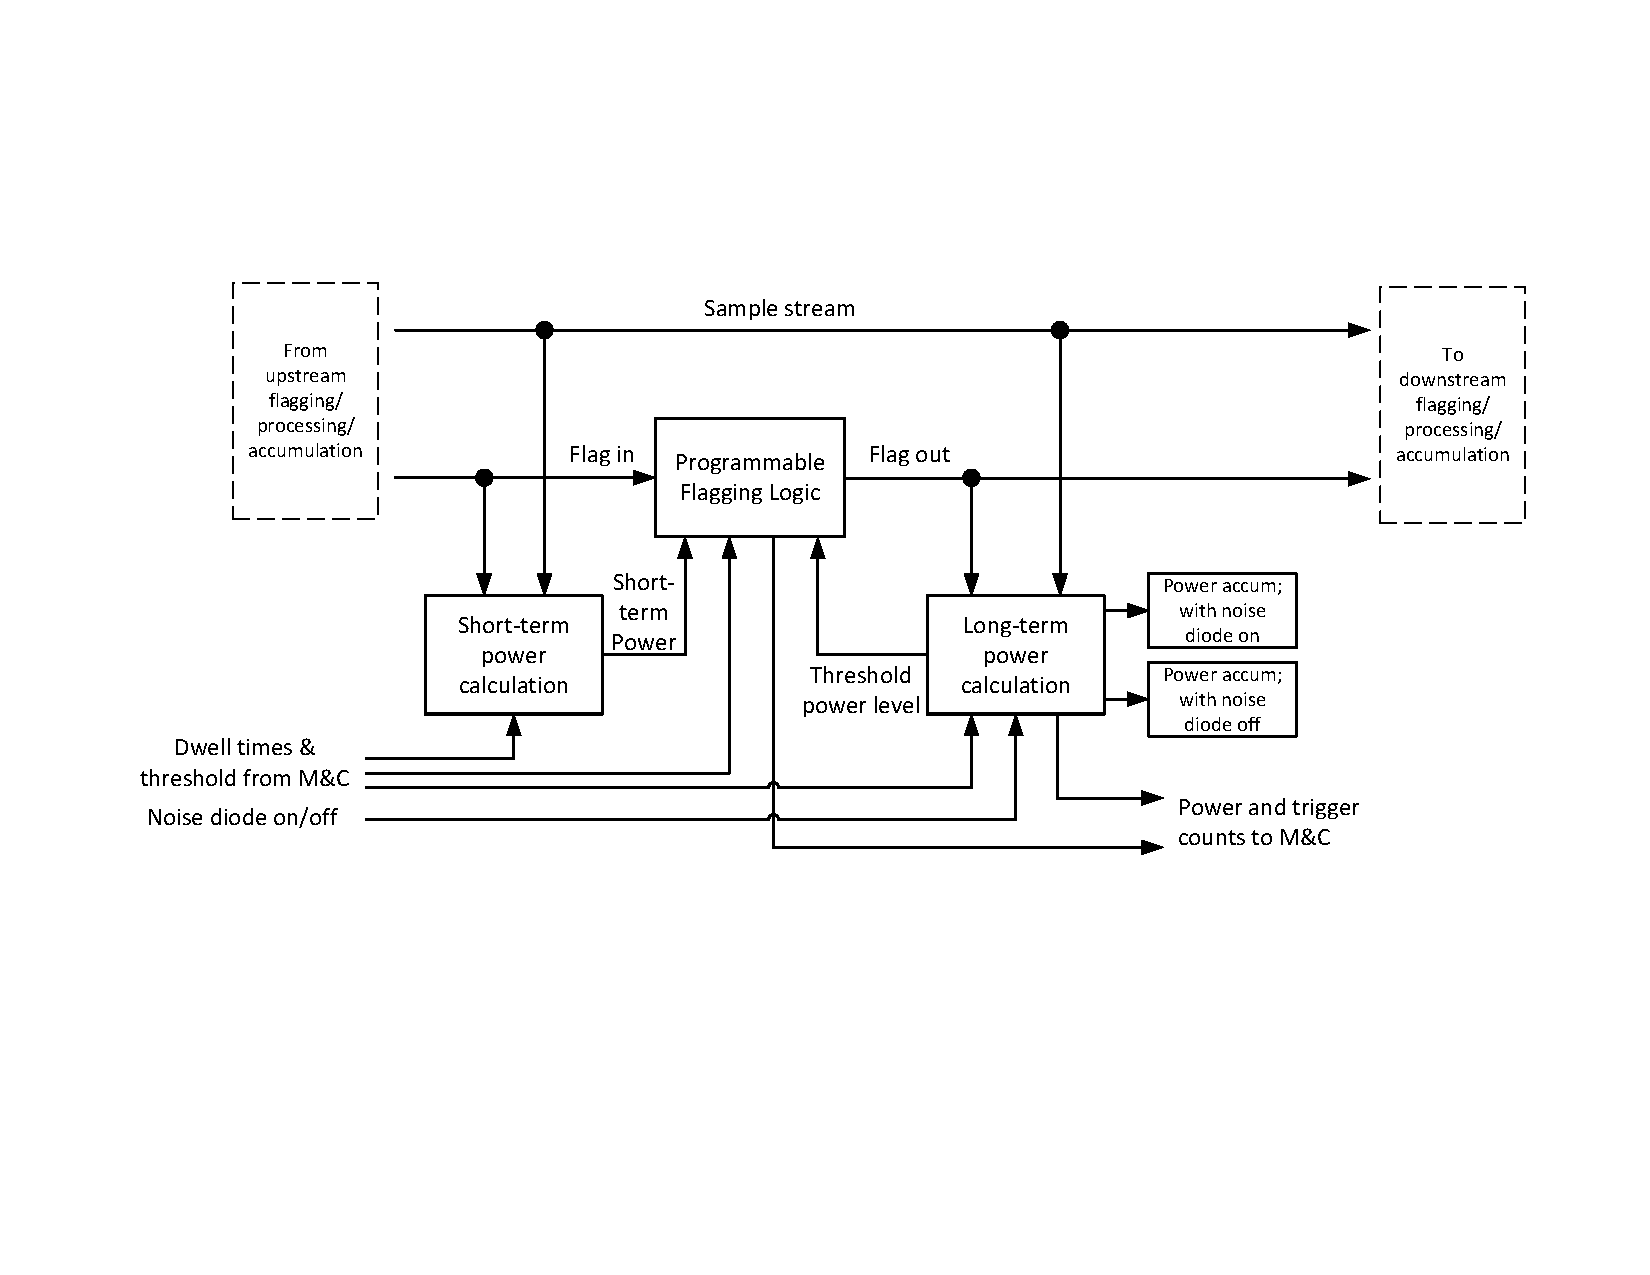
\includegraphics[height=.28\textheight]{figures/RFI_DF_SKA_Mid_CBF.pdf}
    \caption{}
    \label{fig:rfi_df_ska_mid_cbf}
\end{figure}


\subsubsection{Digital : excision in UV domain (Greg)}

GRIDflag \cite{10464448} is a UV-plane-based RFI flagging algorithm designed to enhance the sensitivity and imaging fidelity of radio interferometric observations in the presence of strong and persistent RFI. Unlike traditional methods that flag RFI in the time-channel plane of baselines, GRIDflag operates directly in the UV plane, where multiple baselines sample similar spatial Fourier components redundantly across a regular grid. By statistically comparing UV samples within each grid pixel, GRIDflag identifies and flags RFI-affected points, preserving UV coverage and sensitivity to spatial scales. This approach is particularly effective in mitigating systematic noise introduced by faint RFI, which can otherwise degrade image sensitivity and accuracy. GRIDflag's design allows it to be computationally efficient and adaptable to modern technologies like GPUs, making it well-suited for current and next-generation radio telescopes.

\subsubsection{Digital : Spatial filtering (Greg, Kaushal)}
\begin{itemize}
\item Classic spatial filtering

The core idea is to leverage the spatial diversity of RFI and astronomical signals, along with the unique spatial signatures of interfering sources, to separate and suppress RFI \cite{hellbourg2014radio,hellbourg2016spatial,hellbourg2014rfi}. By estimating the RFI subspace using techniques like Singular Value Decomposition (SVD) and exploiting cyclostationary properties of RFI signals, spatial filters are designed to project received signals onto subspaces orthogonal to the RFI, effectively nulling interference. These filters can be applied either before or after correlation stages in the data processing chain. The technique is particularly valuable for modern radio telescopes, such as LOFAR and EMBRACE, where dense antenna arrays provide numerous redundant measurements, enhancing the precision of RFI mitigation without significantly impacting the desired astronomical signal. This approach helps maintain high fidelity and sensitivity in observations despite increasing RFI challenges from human-made sources.

\item Reference-antenna

A reference antenna can be used to mitigate RFI in real time by providing an accurate estimation of the RFI spatial signature, which can then be used for spatial filtering in radio astronomy. The reference antenna is positioned to specifically capture the RFI without significantly receiving the astronomical signals. This RFI reference signal is correlated with the signals received by the main telescope array, allowing the RFI's spatial signature to be extracted and identified. This information is then used to project out the RFI from the main array's data using spatial filtering techniques, such as subspace projection.

By continuously updating the RFI spatial signature using subspace tracking algorithms, like the Power Method or Rayleigh Quotient Iteration, the system can adapt to changes in the RFI environment in real time, effectively cancelling out the interference without impacting the astronomical signals. This approach is particularly effective for managing multiple RFI sources and dynamically changing interference patterns, enabling high-fidelity observations even in heavily contaminated radio bands\cite{hellbourg2014reference,sardarabadi2015spatial}.

\end{itemize}
\subsubsection{Digital AI/ML} (Greg, Kaushal)
\begin{itemize}
\item Collaborative Signal Subtraction (Greg)

The collaborative approach to RFI mitigation works by establishing a bidirectional communication between radio telescopes and interfering sources, such as cellular networks, to actively share RFI information and cancel interference in real-time. The interfering sources decompose their signals into a compact representation using techniques like the Karhunen–Loève Transform (KLT), which captures the signal's statistical properties independent of time and frequency. This RFI information, including eigenfunctions representing the interference, is periodically shared with the telescope through a low-overhead communication channel.

At the telescope, the received composite signal, which includes both astronomical signals and RFI, is similarly decomposed. The shared RFI characteristics are then used to cancel the interference from the telescope’s data through orthogonal projections in the eigenspace, thereby revealing the clean astronomical signals. This approach significantly reduces communication and computational overhead by prioritizing the sharing of high-impact RFI data and selectively updating the interference model based on its influence on the telescope, thus maintaining high accuracy in signal recovery while managing multiple RFI sources effectively \cite{chakraborty2023collaboration,chakraborty2024low}.

\item Pattern recognition (Greg)
\item External flag generation (RFI monitor?) (Greg)

An RFI detector can provide real-time flags for radio telescopes by using machine learning techniques to automatically identify and classify interference in the radio frequency spectrum. The system described here \cite{9111666} employs a deep neural network (DNN) that processes time-frequency data, detecting and drawing bounding boxes around RFI events. This approach allows the detector to continuously monitor the RF environment and flag novel or anomalous RFI events in real-time. The detected RFI events are flagged based on their spatial, spectral, and temporal characteristics, allowing the telescope to dynamically adjust its data processing pipeline to exclude or compensate for contaminated signals.

By integrating with the telescope’s data stream, the system can provide immediate notifications about RFI, enabling telescopes to respond promptly to interference without manual intervention. This real-time detection capability is particularly useful for maintaining the quality of astronomical observations by preventing the degradation of data due to unwanted interference.

\item Use of higher order statistics (Kaushal)
\end{itemize}